\let\negmedspace\undefined
\let\negthickspace\undefined
\documentclass[journal]{IEEEtran}
\usepackage[a5paper, margin=10mm, onecolumn]{geometry}
\usepackage{tfrupee}

\setlength{\headheight}{1cm}
\setlength{\headsep}{0mm}

\usepackage{gvv-book}
\usepackage{gvv}
\usepackage{cite}
\usepackage{amsmath,amssymb,amsfonts,amsthm}
\usepackage{algorithmic}
\usepackage{graphicx}
\usepackage{textcomp}
\usepackage{xcolor}
\usepackage{txfonts}
\usepackage{listings}
\usepackage{enumitem}
\usepackage{mathtools}
\usepackage{gensymb}
\usepackage{comment}
\usepackage[breaklinks=true]{hyperref}
\usepackage{tkz-euclide} 
\usepackage{listings}

\def\inputGnumericTable{}
\usepackage[latin1]{inputenc}                                
\usepackage{color}                                            
\usepackage{array}                                            
\usepackage{longtable}                                       
\usepackage{calc}                                             
\usepackage{multirow}                                         
\usepackage{hhline}                                           
\usepackage{ifthen}                                           
\usepackage{lscape}

\begin{document}

\bibliographystyle{IEEEtran}
\vspace{3cm}

\title{CHAPTER - 4\\Quadratic Equations}
\author{EE24BTECH11061 - Rohith Sai}

{\let\newpage\relax\maketitle}

\renewcommand{\thefigure}{\theenumi}
\renewcommand{\thetable}{\theenumi}
\setlength{\intextsep}{10pt}

\numberwithin{figure}{enumi}
\renewcommand{\thetable}{\theenumi}

\section*{Exercise : 4.2}
\begin{enumerate}
\item [4.1)] Find the roots of the following equation $2x^2 - x + \frac{1}{8} = 0$\\
\textbf{Solution:} \\
First, we simplify the given equation:
\begin{align}
    2x^2 - x + \frac{1}{8} = 0 \\
    \implies 16x^2 - 8x + 1 = 0
\end{align}

\section*{Newton's Method}
Newton's Method is given by the update formula:
\begin{align}
    x_{n+1} = x_n - \frac{f(x_n)}{f'(x_n)}
\end{align}
where:
\begin{align}
    f(x) = 16x^2 - 8x + 1 \quad \text{and} \quad f'(x) = 32x - 8
\end{align}
The update equation becomes:
\begin{align}
    x_{n+1} = x_n - \frac{16x_n^2 - 8x_n + 1}{32x_n - 8}
\end{align}
Using an initial guess $x_0 = 0.5$, we observe that $x_n$ converges at the 18th iteration to:
\begin{align}
    x = 0.25
\end{align}

\section*{Secant Method}
Alternatively, we can use the Secant Method, which avoids the derivative:
\begin{align}
    x_{n+1} = x_n + f(x_n) \frac{x_n - x_{n-1}}{f(x_n) - f(x_{n-1})}
\end{align}
Taking initial guesses $x_0 = 0.5$ and $x_1 = 0.4$, we observe that $x_n$ converges at the 25th iteration to:
\begin{align}
    x = 0.25
\end{align}
The graph below shows the equation and the root of the equation
\begin{figure}
    \centering
    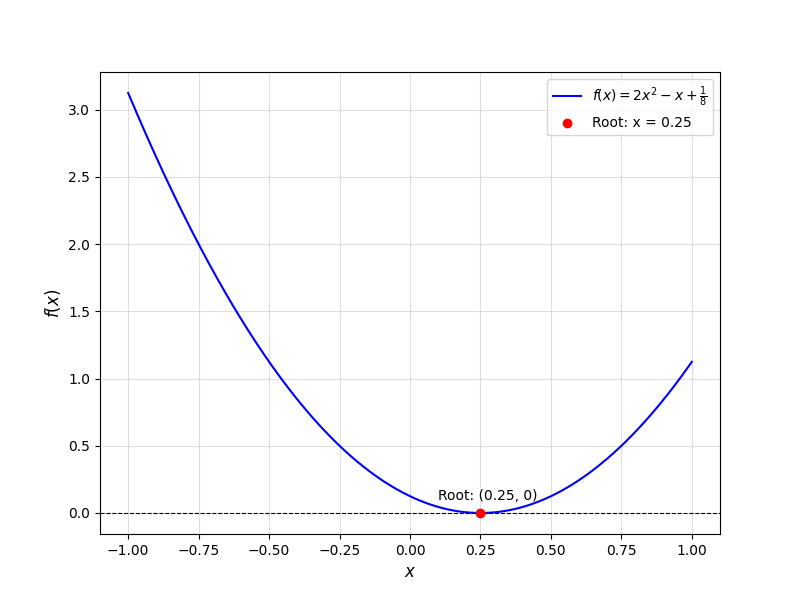
\includegraphics[width=\columnwidth]{figs/fig.png}
\end{figure}

\end{enumerate}
\end{document}
